\subsection{\textit{Bottleneck Adapter}}

Teknik ini memperkenalkan konsep "\textit{tiny-attention}", dibandingkan dengan menambahkan lapisan adaptasi berukuran besar atau melatih ulang seluruh model. Mekanisme ini, meskipun sederhana, memungkinkan setiap posisi dalam sekuens untuk memperhatikan dan memodifikasi keadaan tersembunyinya berdasarkan informasi dari semua posisi lain dalam sekuens \parencite{tinyattention}. Dengan kata lain, setiap elemen dalam sekuens memiliki kemampuan untuk "berkomunikasi" dan "berkoordinasi" dengan elemen lain untuk membentuk representasi yang lebih kaya dan kontekstual.

Salah satu kelebihan dari pendekatan ini adalah fleksibilitas dan dinamikanya. Karena setiap posisi dapat memperhatikan semua posisi lain, model memiliki kapasitas untuk memahami hubungan antar kata dengan lebih baik, terutama hubungan yang bersifat jarak jauh atau kontekstual yang kompleks. Ini memungkinkan model untuk menangkap nuansa dan makna yang mungkin terlewatkan oleh teknik adaptasi lainnya. Arsitektur dari \textit{Bottleneck Adapter} dapat dlihat pada Gambar \ref{fig:tiny-attention}.

\begin{figure}[ht]
    \centering
    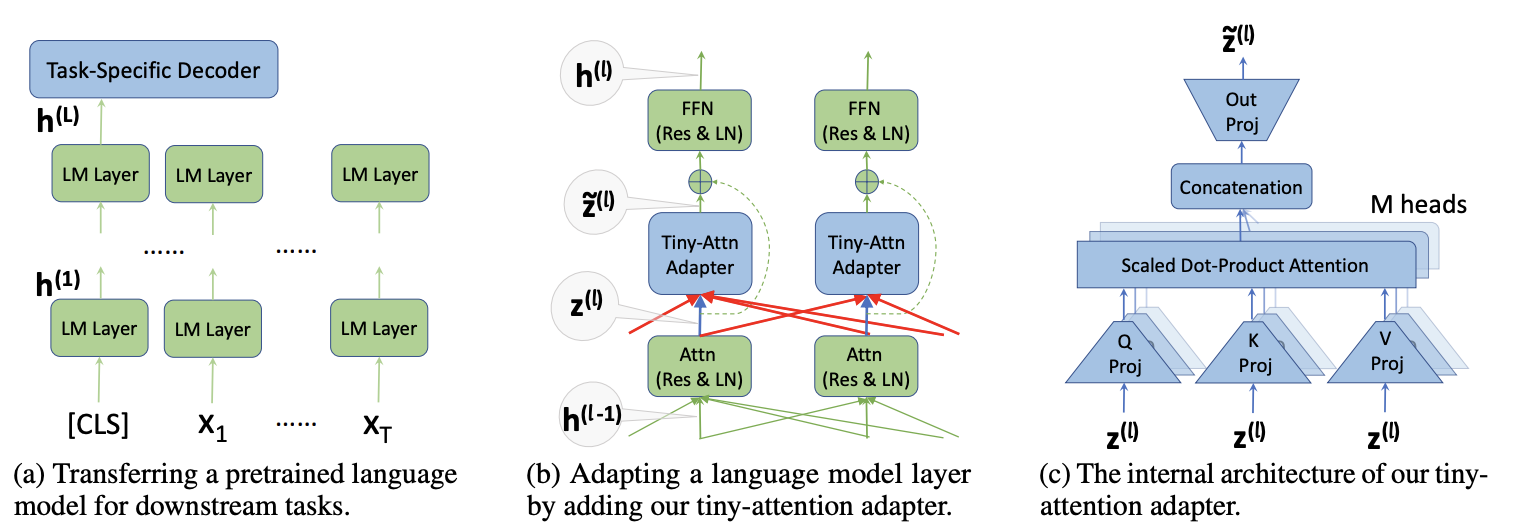
\includegraphics[width=0.8\textwidth]{chapter-2/tiny-attention.png}
    \caption{Arsitektur \textit{Bottleneck Adapter} \parencite{tinyattention}}
    \label{fig:tiny-attention}
\end{figure}


Meskipun pendekatan ini terfokus pada efisiensi parameter, \textit{Bottleneck Adapter} tidak mengorbankan kinerja. Sebaliknya, berkat mekanisme "tiny-attention", teknik ini seringkali mampu mencapai kinerja yang sebanding atau bahkan melampaui metode adaptasi tradisional, meskipun hanya dengan sebagian kecil dari parameter tambahan.
